\documentclass{document_layout}

% Title and author information 
\title{Title of the Paper}
\author{Eduardo Barroso}
\date{\today}

\setabstract{
    This work puts forward a design of multi-component Gabor super-lens that is capable of focusing a wide field of view into a single point.
     In this sense, an array of independent ommatidium composed of sets spherical gradient-index media are capable of focusing light with negligible aberrations similar to that of the Luneburg lens but with reduced overall dimension. 
     The first sections of this work present the design geometric relations and simulates that the design is viable with numerical simulations based on the Lagrangian optics formalism. In the succeeding chapter, optimizations on the super-lens and individual lenses are presented. 
     The former consists on careful implementations of geometrical and optical implications. For the latter, in order to minimize individual lens aberrations, the team introduces a variant of the Gutman lens that has three degrees of freedom giving rise to a refined optimization. 
     Finnaly, numerical results are then presented with ray-optics, wave-optics simulations and a experimental result validates the findings. The closing sections of the paper are reserved for applications of such design in photonics, lithographic technologies, medicine, machine vision, telecommunication antennas and compound lens cameras. 
}

% Begin the document
\begin{document}

\maketitle

    
\section*{Introduction}
\label{sec:introduction}
Optical systems that focus light in a single point have substantial relevance in many engineering fields such as biomedical, photography, lithography and telecommunication \cite{machikhin2015double,bn2022application,brunner1997impact,bjorkqvist2019additive}. By concentrating light into a single point it is possible to form sharp images, print precise patterns in semiconductors \footnote{A foundational manufacturing technology for chips} and direct with high precision radio waves. Thus, the optimization of optical systems with precise focal abilities can yield huge benefits in optics related industries. One example of such system is the Luneburg lens, this is a spherical gradient index (GRIN) distribution that yields analytical ray tracing solutions without aberration in a point of the surface of the lens. \\ 

Although Luneburg lenses are aberration free, they have practical downsides. The spherical shape can be difficult to manufacture when considering wide fields of view leading to dimensional limitations \footnote{A study has shown that if the image resolution of compound  eyes increases to the same level as the human’s single aperture eye, the radius of the overall lens would be at least 1 m \cite{kirschfeld1976resolution}}. In addition, the lens has a continuous distribution, this means that the surface of the lens must have a refractive index equal to its surroundings - another huge manufacturing challenge. In order to overcome such practical downsides, it is possible to conceive the idea of super-lens composed of smaller, individual spherical lenses with distinct GRIN distributions that can concentrate a wide field of view into an aberration-free point. The design presented in the paper consists of two GRIN distributions: the Luneburg lens and a variation of the Gutman lens.\\

When designing optical systems, it is convenient to use ray-tracing to monitor the behavior of light inside the system. In 2021 Jesus Gomez et. al published a paper that puts forward a ray-tracing methods using Fermat's invariant \cite{GomezCorrea21}. Such paper discussed how the Lagrangian formulation of optics gives rise to Fermat's constant which in turn can be used to formulate a very elegant ray-tracing algorithm that unlike traditional methods; can be generalized to many systems. The algorithm consists on calculating Fermat´s invariant $k$ at the beginning of the propagation and then using it to calculate the angle of diffraction at any point along the trajectory. This describes how the light-beam bends inside the GRIN media. Both its simplicity and accuracy makes it particularly convenient when designing optical systems. Biomimicry is also favorable starting point for engineering designs. By exploiting billions of years of evolution many fields of engineering have flourished. Thus we now proceed to present our design inspired by nature´s eyes. \\

\section{Super-Lens Design}
\subsection{Compound eyes and the Gabor Super-lens}
When designing optical systems, there usually exists a compromise between two optical properties the field of view (FOV) and resolution. The resolution is related to the ability of the system to minimize aberrations. The field of view is defined as the angular aperture of a frame imaged by the optical system of interest, i.e. the solid angle that spans frame being captured \cite{dobbert2006matchmoving}.\\

Insects such as moths have evolved to have a wide field of view in order to detect predators incoming from various directions. Their eyes are able to achieve this because they are composed of many individual ommatidiums oriented in a semi-sphere as shown in figure \ref{fig:Superposition_Compound_eye}[b]. In this sense, they are termed compound eyes. Compound eyes are natural imaging systems that consist of many independent lenses that act as a system in order to produce images.  An array of the individual lenses is named ommatidium, formally defined as the minimum imaging unit of compound eyes \cite{cheng2019review}. In particular, the field of biological optics distinguishes between three types of compound eyes \cite{volkel2003miniaturized}. These are the apposition \cite{fallah2010mtf}, superposition \cite{greiner2004retinal} and neural superposition compound eyes \cite{frederiksen2008visual}. \\

The design presented in this work closely resembles the refracting superposition compound eye in the sense that all ommatidium focus light into a single point. This type of compound eye are found in insect species such as moths (Figure \ref{fig:Superposition_Compound_eye}).  In particular, this type of compound eyes are characterized for having the best imaging resolution with research reporting resolutions up to ten times higher than that of the apposition compound eye \cite{stollberg2009gabor,kirschfeld1974absolute}. \\

\begin{figure}[H]
    \centering
    \begin{subfigure}[t]{0.48\columnwidth} % Adjust width to fit within column
        \centering
        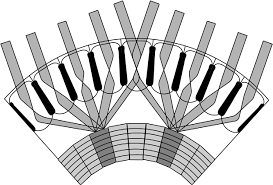
\includegraphics[width=\textwidth]{Figures/refracting superposition compound eye.png}% Ensure correct width
        \label{fig:S_Compound_eye}
    \end{subfigure}
    \hfill
    \begin{subfigure}[t]{0.48\columnwidth} % Adjust width for the second image
        \centering
        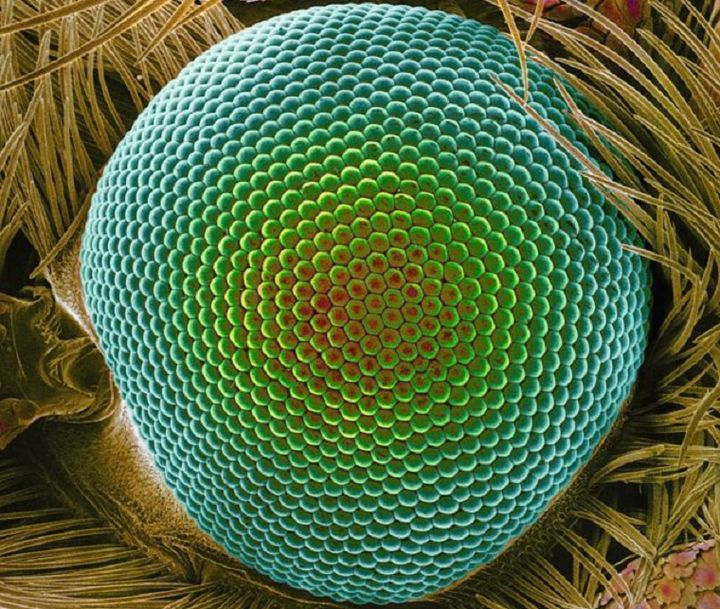
\includegraphics[width=\textwidth]{Figures/Moth_Compound eye.jpg} % Ensure correct width
        \label{fig:Moth}
    \end{subfigure}
    \caption{Transversal view of the superposition compound eye (left); Moth superposition compound eye (right).}
    \label{fig:Superposition_Compound_eye}
\end{figure}



In micro-optics, the practical implementation of superposition compound eyes are termed Gabor super-lenses \cite{stollberg2009gabor} named after Dennis Gabor who in 1940 introduced the concept application for micro-cameras \cite{DGaborSL}. As presented in figure \ref{fig:Gabor design}, the basic Gabor super-lens consists of two micro lenses arrays (MLAs) where the separation is dictated by each layer focal distance. In this sense, the work introduces a Gabor super-lens consisting of three layered micro lens array. In the following section the geometrical considerations are presented.\\ 

\begin{figure}[H]
    \centering
    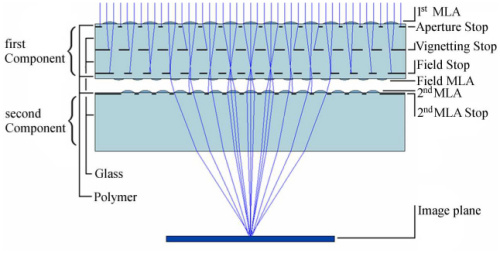
\includegraphics[scale=0.60]{Figures/Gabor-Superlens.jpeg}
    \caption{Gabor super-lens design \cite{stollberg2009gabor} .}
    \label{fig:Gabor design}
\end{figure}

\subsection{Geometric Parameters of the Design}
In this section, a proposal for the Gabor super-lens is presented. The design is built in order to obtain aberration free system, capture a wide field of view and minimize the system´s focal distance. Furthermore, the design consists on a clever arrangement of a three layered ommatidium. Each layer is characterized by its own characteristic curvature that is determined by the focal distance of the structure and the radius of the individual lenses.\\

Consider the structure of the super-lens in the $y-z$ plane with a focal length $f_t$. The lenses in the first layer array (FLA1) have a focal length $f_1$ and a radius $R_1^0 = R_1^n$, where the lower and upper scripts indicate the layer and number of lens inside the array respectively. The center of lenses in FLA1 lie on a vertical line $z=0$ with coordenates $(zc_1^n,yc_1^n)$, where
\begin{equation}
    zc_1^n = 0 \hspace{0.5cm}\&\hspace{0.5cm} yc_1^n = 2nR_1^n ,
\end{equation}
and n is an integer, which has a variation of $-\frac{m-1}{2}\ge n \le \frac{m-1}{2}$. \\

In this case, $m$ is a positive, odd integer that represents the total number of ommatidium arrays. Assuming that rays come from infinity, the rays passing through lenses in FLA1 will focus at the point $P_1=(f_1,yc_1^n)$,as shown in figure \ref{fig:design}. \\

\begin{figure}[H]
    \centering
    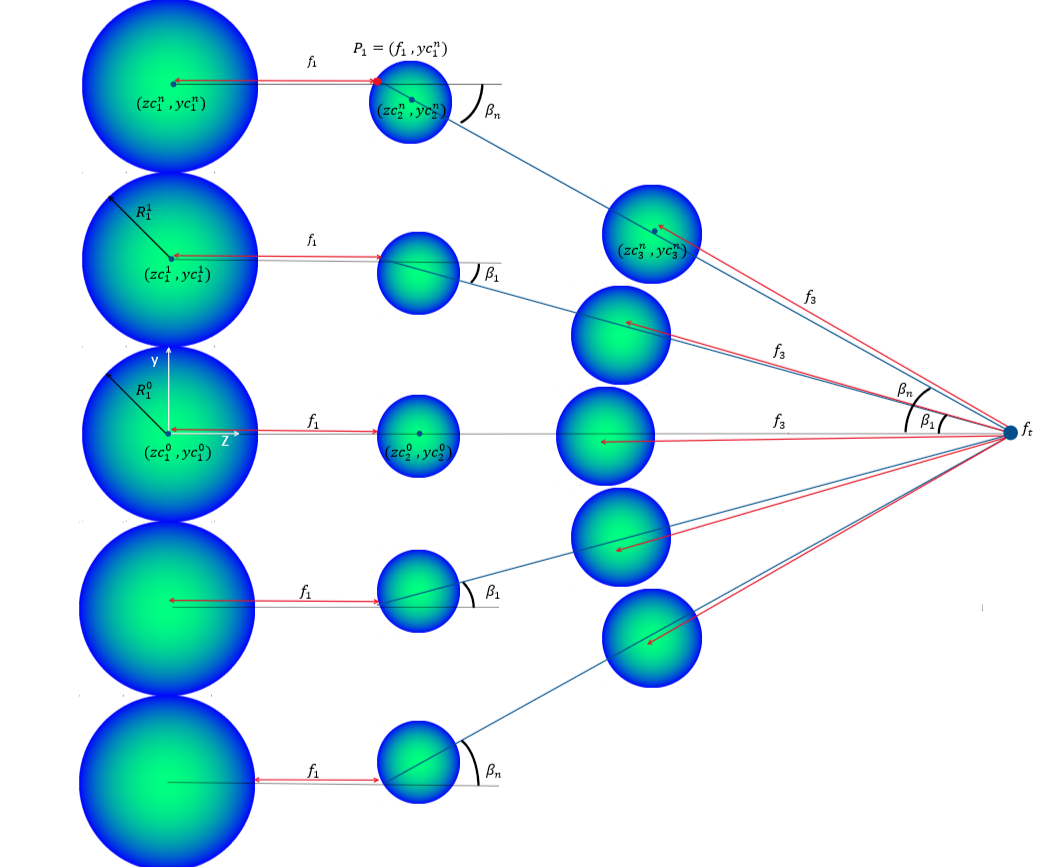
\includegraphics[scale=0.40]{Figures/Superlens_Design_Parameters.png}
    \caption{Super-lens parameters and design.}
    \label{fig:design} 
\end{figure}

The main function of FLA2 is to divert the field from FLA1 in such a way that the center ray will pass through the point $(f_t,0)$. It is known that by placing a source of light on the surface of the Luneburg lens with refractive index $n(r) = \sqrt{2-r^2}$, the field will propagate in the direction given by the angle $\beta_n$, obtaining parallel rays (see figure XXX). The angle $\beta_n$ is given by
\begin{equation}
    \beta_n = arctan(\frac{y_n}{f_1-f_t}).
\end{equation}

In order to ensure the proper diversion, the center of the lenses in FLA2 $(zc_2^n,yc_2^n)$ must be centered in the position

\begin{equation}
\begin{split}
    zc_2^n &= f_1 + R_2^n*cos(\beta_n) \\
    yc_2^n &= yc_1^n - R_2^n*sin(\beta_n),
\end{split}
\end{equation}
where $R_2^n$ is the radius of the Luneburg lenses of FLA2. Note that the centers of these lenses form a curve. \\

The FLA3 must guarantee focus on the point $(f_t,0)$. For this to be possible, the FLA3 lenses must be centered on a point on the line conecting the points $(f_1,yc_1^n)$ and $(f_t,0)$. Their center depends on their focal distance $(f_3)$ and the analytic geometric relation yields
\begin{equation}
\begin{split}
    zc_3^n &= f_t - f_3*cos(\beta_n) \\
    yc_3^n &= f_3*sin(\beta_n). 
    \end{split}
\end{equation}

Note that the radii on FLA3 are not free parameters \footnote{The plural noun results because the each lens is free to have its own radius.}, rather they are restrained by the non linear increment of $\beta_n$ since two lenses cannot overlap. 

\subsection{GRIN Distributions in focal lenses arrays}
Once the geometric parameters of the Gabor lens have been defined, it is important to define the GRIN of the lenses for each FLA. For the FLA1 and FLA3, the GRIN is given by 
\begin{equation}
    n(r) = \left[\frac{(R^2+f^2-\alpha r^2)}{f}\right]^\beta,
\end{equation}

where $f$ is an focal distance factor, $\alpha$ corrects a radial contribution and $beta$ is a non-paraxial correction factor with positive integer values for the 3 parameters. Their value will be obtained in a optimization process. \\

Finally, the lenses in FLA2 are modeled as Luneburg lenses. However a proper normalization factor needs to be introduced for $R_2^n \neq 1$. The normalized GRIN distribution is given by
\begin{equation}
    n(r) = \sqrt{2-\frac{r}{R_2}}.
\end{equation}



\section{Design: A proof of concept}
The proof of concept consists on building a numerical, two-dimensional simulation of the super-lens. Theoretically, paraxial beams incident on each individual ommatidium should focus light onto a single point. As shown in figure (\ref{fig:Superlens POC}), the design is not capable of obtaining free aberration on the system focal point. This is highly in part because the lenses in the first and third layer have spherical aberrations. In particular, the further their focal points the higher the aberration. Thus, a strict optimization is needed in order to obtained the desired results for this work. \\

\begin{figure}[H]
    \centering
    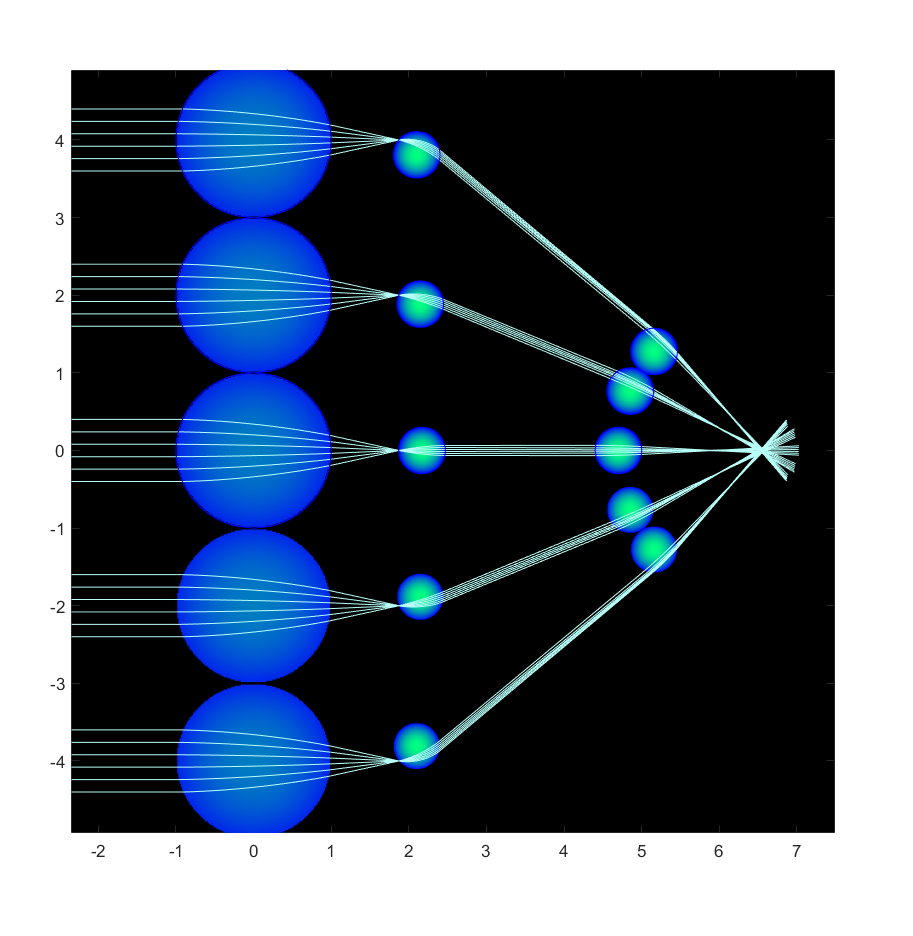
\includegraphics[width=\columnwidth]{Figures/MYSuperplens_POC.png}
    \caption{Two dimensional simulation of the proposed super-lens design to present the proof of concept.}
    \label{fig:Superlens POC}
\end{figure}


Also a three dimensional rendering is presented. With this design, the practical applications disused in the opening lines of the work can be exploited. 

\begin{figure}[H]
    \centering
    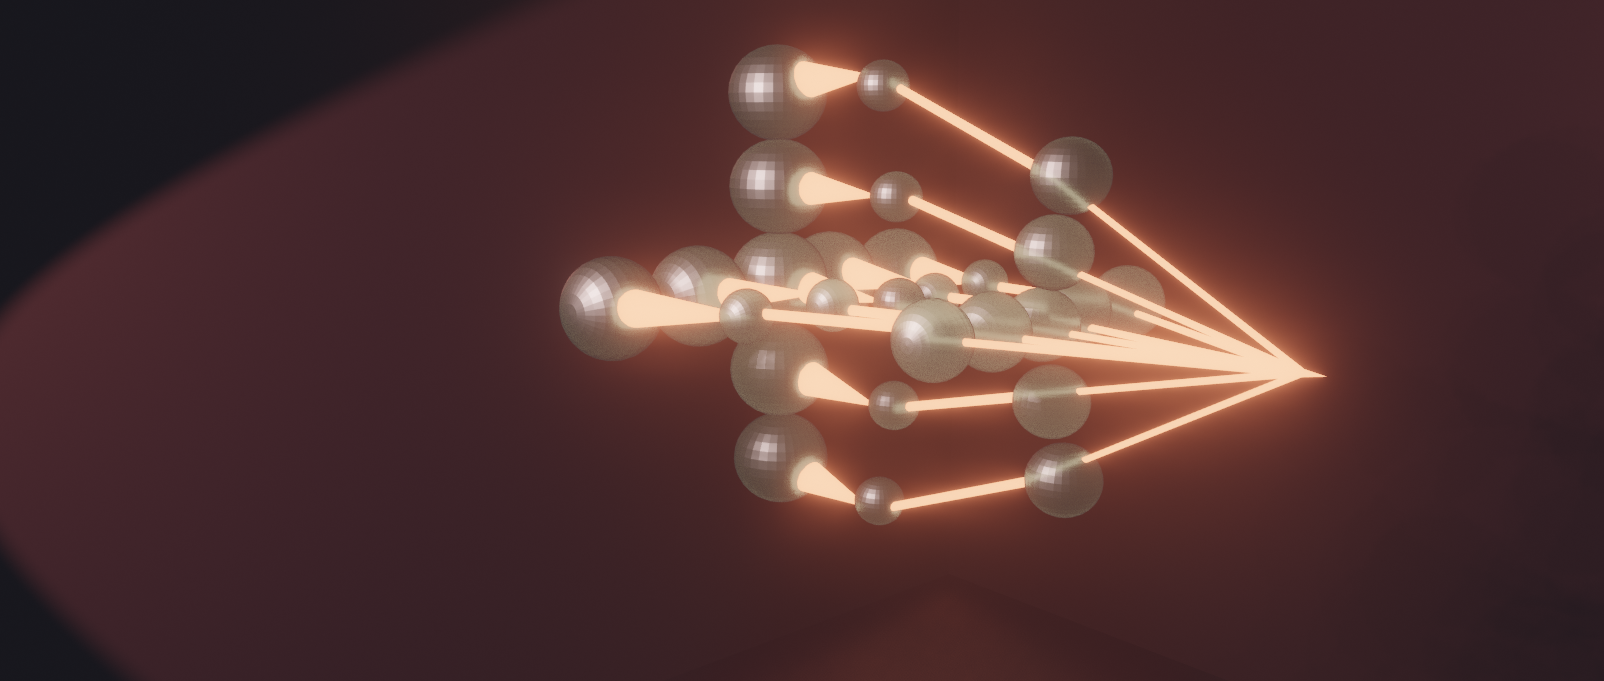
\includegraphics[width=\columnwidth]{Figures/Side-front-superlens.png}
    \caption{Three dimensional model of the proposed super-lens design.}
    \label{fig:Superlens design}
\end{figure}

\section{Numerical Optimization and Results}
In order to connect the continuous classical models of light with this work discrete numerical designs we start by comparing the numerical results for aberrations in the normalized Luneburg lens with analytic solutions. \footnote{Analytically, Luneburg conjecture yields zero aberration}. Thus, aberrations in the super-lens in the order of the aberrations in the Luneburg lens are acceptable and reported as free aberrations. \\

\subsection{Relevant Design parameters and relations}
In order to make a proper optimization of the super-lens, its necessary to understand the relations between the system parameters. Firstly, note that the  focal distance of the first array of lenses determines the spread of the parameter $\beta_n$. In addition, larger values for this spread allow for bigger radius on the third layer $R_3^n$  which leads to smaller values of aberrations (Err) as a result of,
\begin{equation}
    Err \propto \frac{f}{R}
\end{equation}

There exists another relation between the maximum height of incidence (H) in the third array and the radius of the second array of lenses. The smaller the radius, the lower the rays leading to smaller aberrations of the third array and overall system. This relation can also be understood with optical magnification. Thus, it is important to respect $R_2^n < R_3^n$.
\begin{equation}
    Err \propto H_f \propto \frac{f}{R}
\end{equation}

Finally, the relation to the spread on $\beta_n$  and the focal distance of the super-lens dictates to minimize the spacing between the second and third layer without sacrificing too much height (H). Thus, for the last layer, it is also convenient to set a limit on the ratio

\begin{equation}
    Err  \propto \frac{H_f}{R} \propto  \frac{1}{ft-f_1+f_3}.
    \label{eq:errproptoh}
\end{equation}


\subsection{Individual lens Optimization}
The Luneburg conjecture leads to the conclusion that each lens can have zero aberration for a finite focal length. Furthermore, the Gutman lens, whose refractive index profile is given by
\begin{equation}
    n(r) = \sqrt{\frac{R^2+f^2-r^2}{f^2}},
\end{equation}
has the property of focusing rays outside the lens but with spherical aberration. To overcome such aberrations it is possible to introduce correction factors to the distribution that help minimize such aberrations. This has benn done previusly by Zhao. et al \cite{zhao} but the results they reported where false and presented aberrations in our numerical simulations. Thus, in order to make a proper optimization we introduced the following distribution with 3 degrees of freedom: $\alpha,\beta,R$ and
\begin{equation}
    n(r) = [\frac{R^2+f^2-\alpha r^2}{f^2}]^\beta.
\end{equation}

Introducing the factor $\beta$ allows for control over the aberrations of rays outside the paraxial height. This is important because the objective is to capture a wide FOV. In particular, the optimization of beta becomes relevant in the first layer because $H_f=R_1^n$ and the relation with the aberration given by \ref{eq:errproptoh}. For the first lens array we obtained the following results. 
\begin{center}
    \begin{table}[H]
    \resizebox{\columnwidth}{!}{ % Scale to column width
    \begin{tabular}{|c|c|c|c|c|c|}
    \hline
    \textbf{R} & \textbf{$\alpha$} & \textbf{$\beta$} & \textbf{$f$} & \textbf{$z_{ave}$} & \textbf{Err} \\ \hline
    $R_1^n=1$    & 0.86              & 0.5285              & 1.2315          & 1.3              & 9.3e-4        \\ \hline
    \end{tabular}
    } % End resizebox
    \end{table}
\end{center}


Note that, our numerical optimizations have limits and strongly depend on the computing power and discretization available. Its worth mentioning that the latter results are obtained with a step size L = 0.00005 \footnote{In a unit radius, the center ray travels 40,000 steps. }. In this regime, the numerical aberrations for the Luneburg lens lie on the order of e-4, meaning the super-lens presented has to present aberrations of this same order.\\

The focal distance of the system is set to $6 [r_{units}]$. This is related to the optimization the work wishes to present. To optimize the spatial dimension of the problem, its realistic to propose a $60\%$ reduction. This means that a wave front of 10 units is focused on 6 rather than 10 in the case of the lunemburg lens i.e $f_t = 6 [units]$. \\

Starting from the first layer, with the radius of the lenses unitary, the focal distance is $f_1 = z_ave1=1.3$.  In order to maximize the individual radius of the third layer $R_3^n$, a geometrical relation can be implemented so that all the space is covered while the lenses still lie on the circumference of the curve characteristic of the third layer. To do so, its necessary to fix the radius center lens. For our design we choose $R_3^0 = 0.439$ so that $R_3^1 =R_3^2 = 0.265$. One last optimization consists on finding the optimal GRIN distribution for the third layer lenses. The results obtained are the following.

\begin{center}
    \begin{table}[H]
    \resizebox{\columnwidth}{!}{ % Scale to column widt
    \begin{tabular}{|c|c|c|c|c|c|}
    \hline
    \textbf{R}         & \textbf{$\alpha$} & \textbf{$\beta$} & \textbf{$f$} & \textbf{$z_ave$} & \textbf{Err} \\ \hline
    $R_3^0=0.439$      & 0.745             & 0.5              & 1.049        & 1.7              & 0.001        \\ \hline
    $R_3^1=R_3^2=0.26$ & 0.779             & 0.5              & 0.764        & 1.7              & 0.009        \\ \hline
    \end{tabular}
    } % End resizebox
    \end{table}
\end{center}

The full ensemble of the super lens gives a total aberration of 0.03. This means that the optimization with the specific characteristics presents aberrations with three orders of magnitude greater than perfect focus. The system is presented in figure \ref{fig:superlens_v1}

\begin{figure}[H]
    \centering
    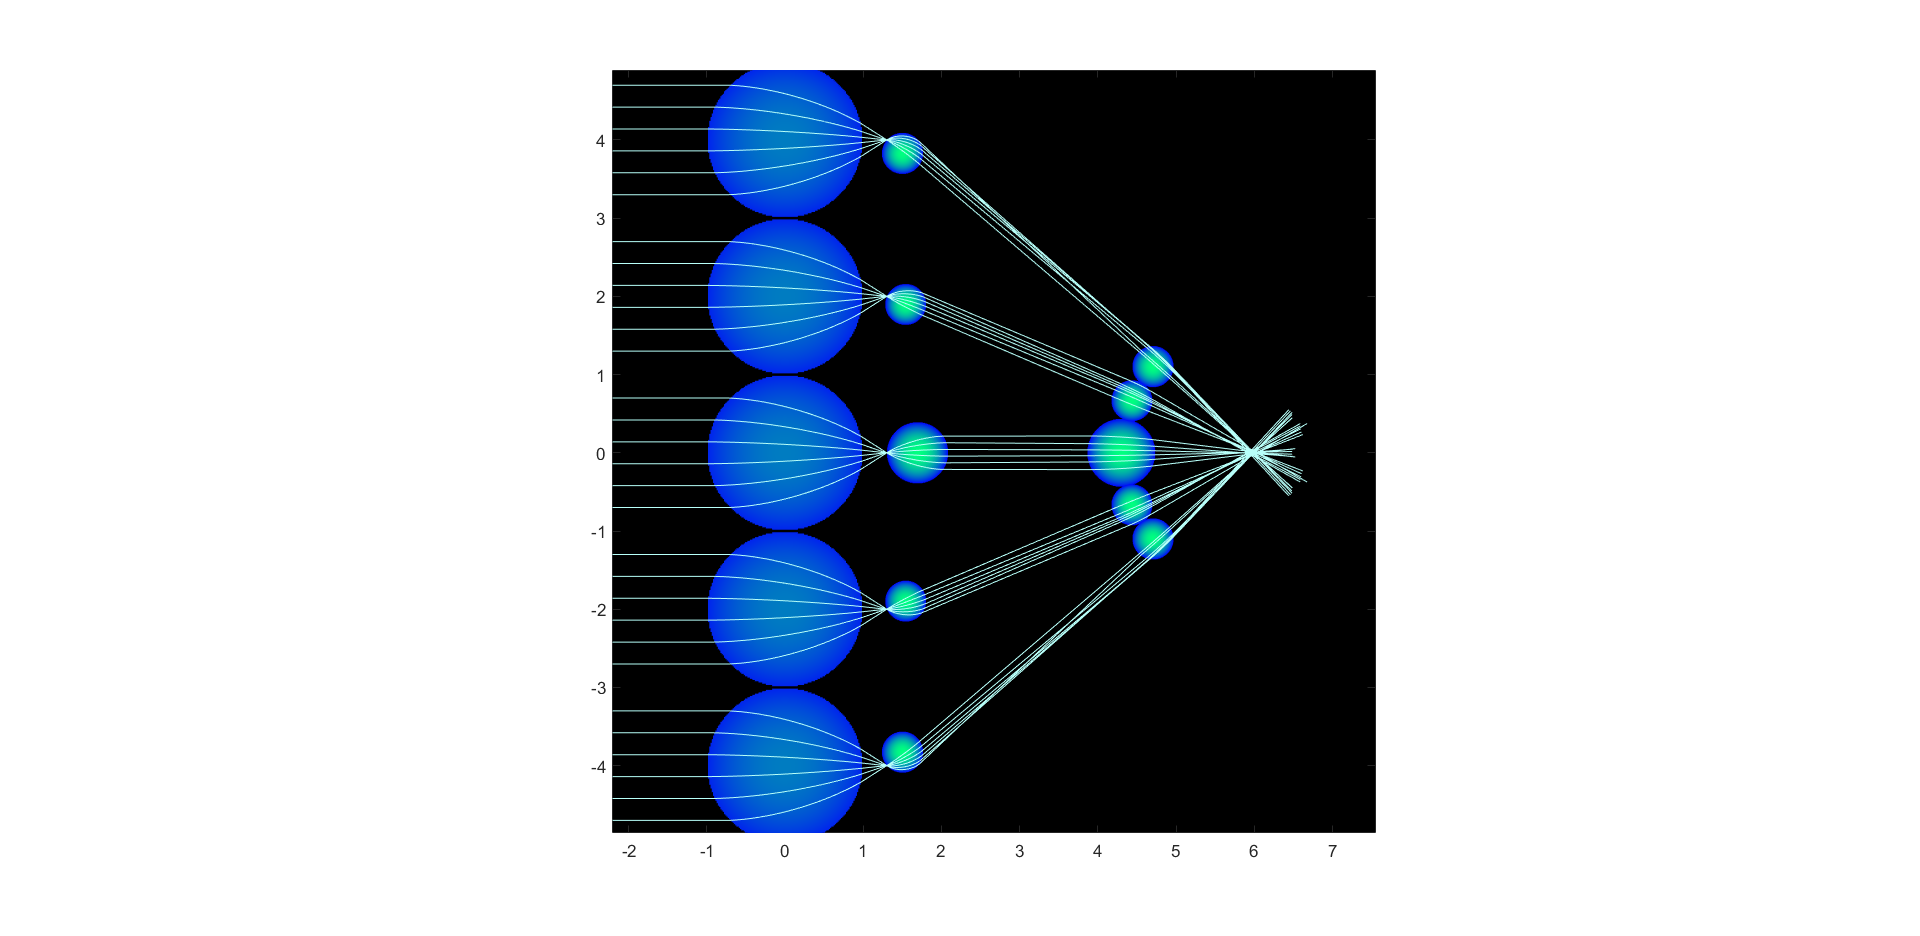
\includegraphics[width=\columnwidth]{Figures/MYSuperlens_final.png}
    \caption{Super-lens distribution}
    \label{fig:superlens_v1}
\end{figure}

\section{Applications}
Imaging systems with a large FOV exhibit exceptional medical, civilian and military applications. In medicine, such systems yield promising results with endoscopies and odontotherapy [16,18]. Regarding civilian and military applications some examples include machine vision and security protection \cite{davis2009bio,duparre2007latest}.\\

\section{Conclusion}
Plasmonic structures work very well when amplifying electromagnetic modes. Furthermore, the work shows that these structures can be present in many distinct optical structures that have different parameters. With the help of analytic modeling, it is possible to design a structure to amplify electromagnetic modes of interest. By evaluating the engineering problems that come with this phenomena, its a mere certainty that this technology is set to become a pinnacle in the current mainstream of quantum technologies.\\


% References
\printbibliography

\end{document}